Трек посвященный воспроизводимости в ML. 
Много разговоров о том
\begin{itemize}
    \item В чем схожесть и отличия обычного процесса разработки ПО и процесса разработки ML моделей
    \item Какие инструменты и подходы, используемые при классической разработке ПО, можно переиспользовать при разработке ML продуктов
    \item Каким образом можно добиться воспроизводимости
\end{itemize}

\begin{remark}
    Наши \href{https://paper.dropbox.com/doc/Reproducible-Research-Draft--A7_r_i5_5DxZO4k9GQMzGWu3AQ-AfvEwFDcTF6lG0nWrdPWj}{рекомендации}.
\end{remark}

\section{Machine Learning REPA in Action}

\textbf{Video:}~\url{https://youtu.be/sZTO6LihuAM} \\

Доклад про lessons learned и good practices, которые позволяют сделать процесс разработки ML моделей воспроизводимым. \\

Time-to-market время при разработке новой модели можно сильно уменьшить если есть следующие ключевые компоненты:
\begin{figure}[ht]
    \centering
    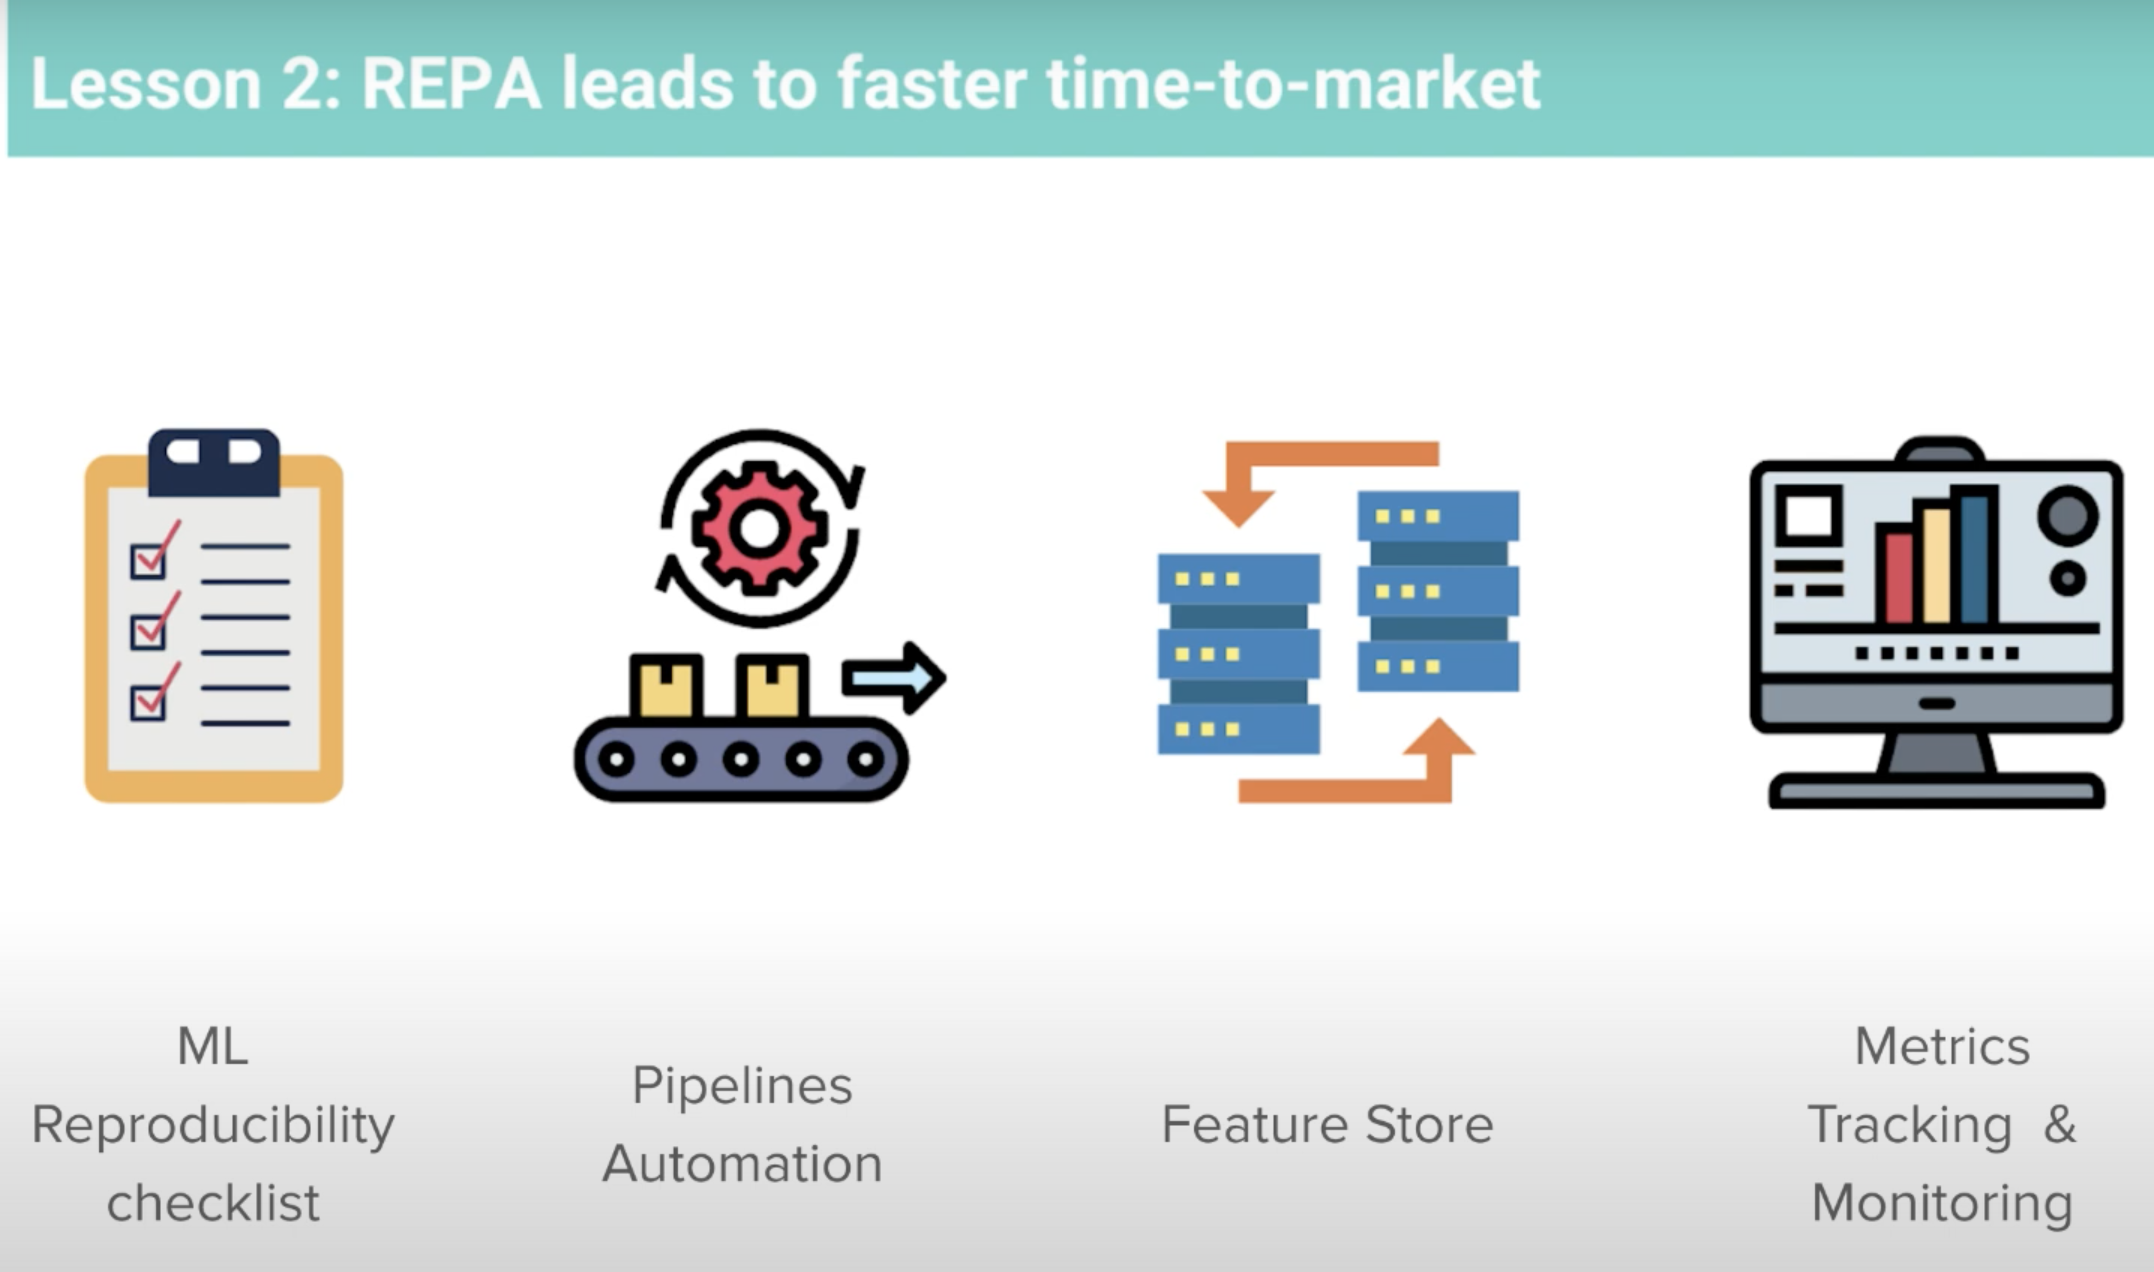
\includegraphics[width=0.8\linewidth]{images/repa.png}
\end{figure}

\subsection{ML Reproducibility checklist}

\begin{enumerate}
    \item Environment dependencies control --- нужно всегда трекать зависимости (версии баблиотек итд)
    \item Code version control --- использовать git для разработки (код ревью экспериментов)
    \item Control run params
    \item Automated pipelines --- собирать пайплайны для обеспечения воспроизводимости
    \item Artifacts version control --- например, трекать версии моделей которые получаются на выходе
    \item Experiments results tracking --- сохранять результаты экспериментов (метрики/артифакты)
    \item Automated CI/CD --- авто-тесты/автоматическая выкатка в прод
\end{enumerate}

\subsection{Good Practices}

\paragraph{Project Organization} Во всех ML проектах команды должна быть похожая структура - это позволяет проще кооперироваться.

В качестве примера структуры ML проекта приводят Cookiecutter Data Science\footnote{\url{https://drivendata.github.io/cookiecutter-data-science/}}.

\paragraph{Task Tracking} Для любого изменения в коде должна быть соотвествующая задачка в таск-трекере.

\paragraph{Documentation} Как минимум в папках с проектом должны быть README.md файлы, в которых кратко описаны основные моменты.

Не стоит забывать и про документацию в confluence.

\paragraph{Testing} Нельзя пренебрегать тестированием (см. Раздел~\ref{sec:testing_ds}).

\section{[MTS] Software engineering life hacks for Data Science}

\textbf{Video:}~\url{https://youtu.be/i-SrzrzpieI} \\

В данном докладе говорилось по большому счету о том же, что есть в наших рекомендациях к воспроизводимости:

\begin{itemize}
    \item Упорядоченный репозиторий
    \item Чистый код (прямая отсылка к книжке)
    \item Рефакторинг
    \item Работа в отдельных ветках и обязательное код ревью. 
        
        Во время ревью следует особое внимание уделить следующим аспектам
        \begin{itemize}
            \item DS ошибки
            \item Воспроизводимость
            \item Ошибки разработки
        \end{itemize}
        
    \item Полезные расширения для Jupyter
        \begin{itemize}
            \item Extensions\footnote{\url{https://github.com/ipython-contrib/jupyter_contrib_nbextensions}} - Execute time, Autopep8, Table of Contents, Collapsible Headings
            \item Papermil\footnote{\url{https://github.com/nteract/papermill}} - инструмент для параметризации и удобного запуска ноутбуков.
            
            Позволяет удобно запустить ноутбук с заданными параметрами.
        \end{itemize}
\end{itemize}

\section{[OK.ru] Reproducibility is not a pain anymore!}

\textbf{Video:}~\url{https://youtu.be/arTk1YvgRls} \\

\begin{center}
    ML модель = Данные + Код + Зависимости
\end{center}

По большому счету повторение предыдущего доклада Миши

\begin{figure}[ht]
    \centering
    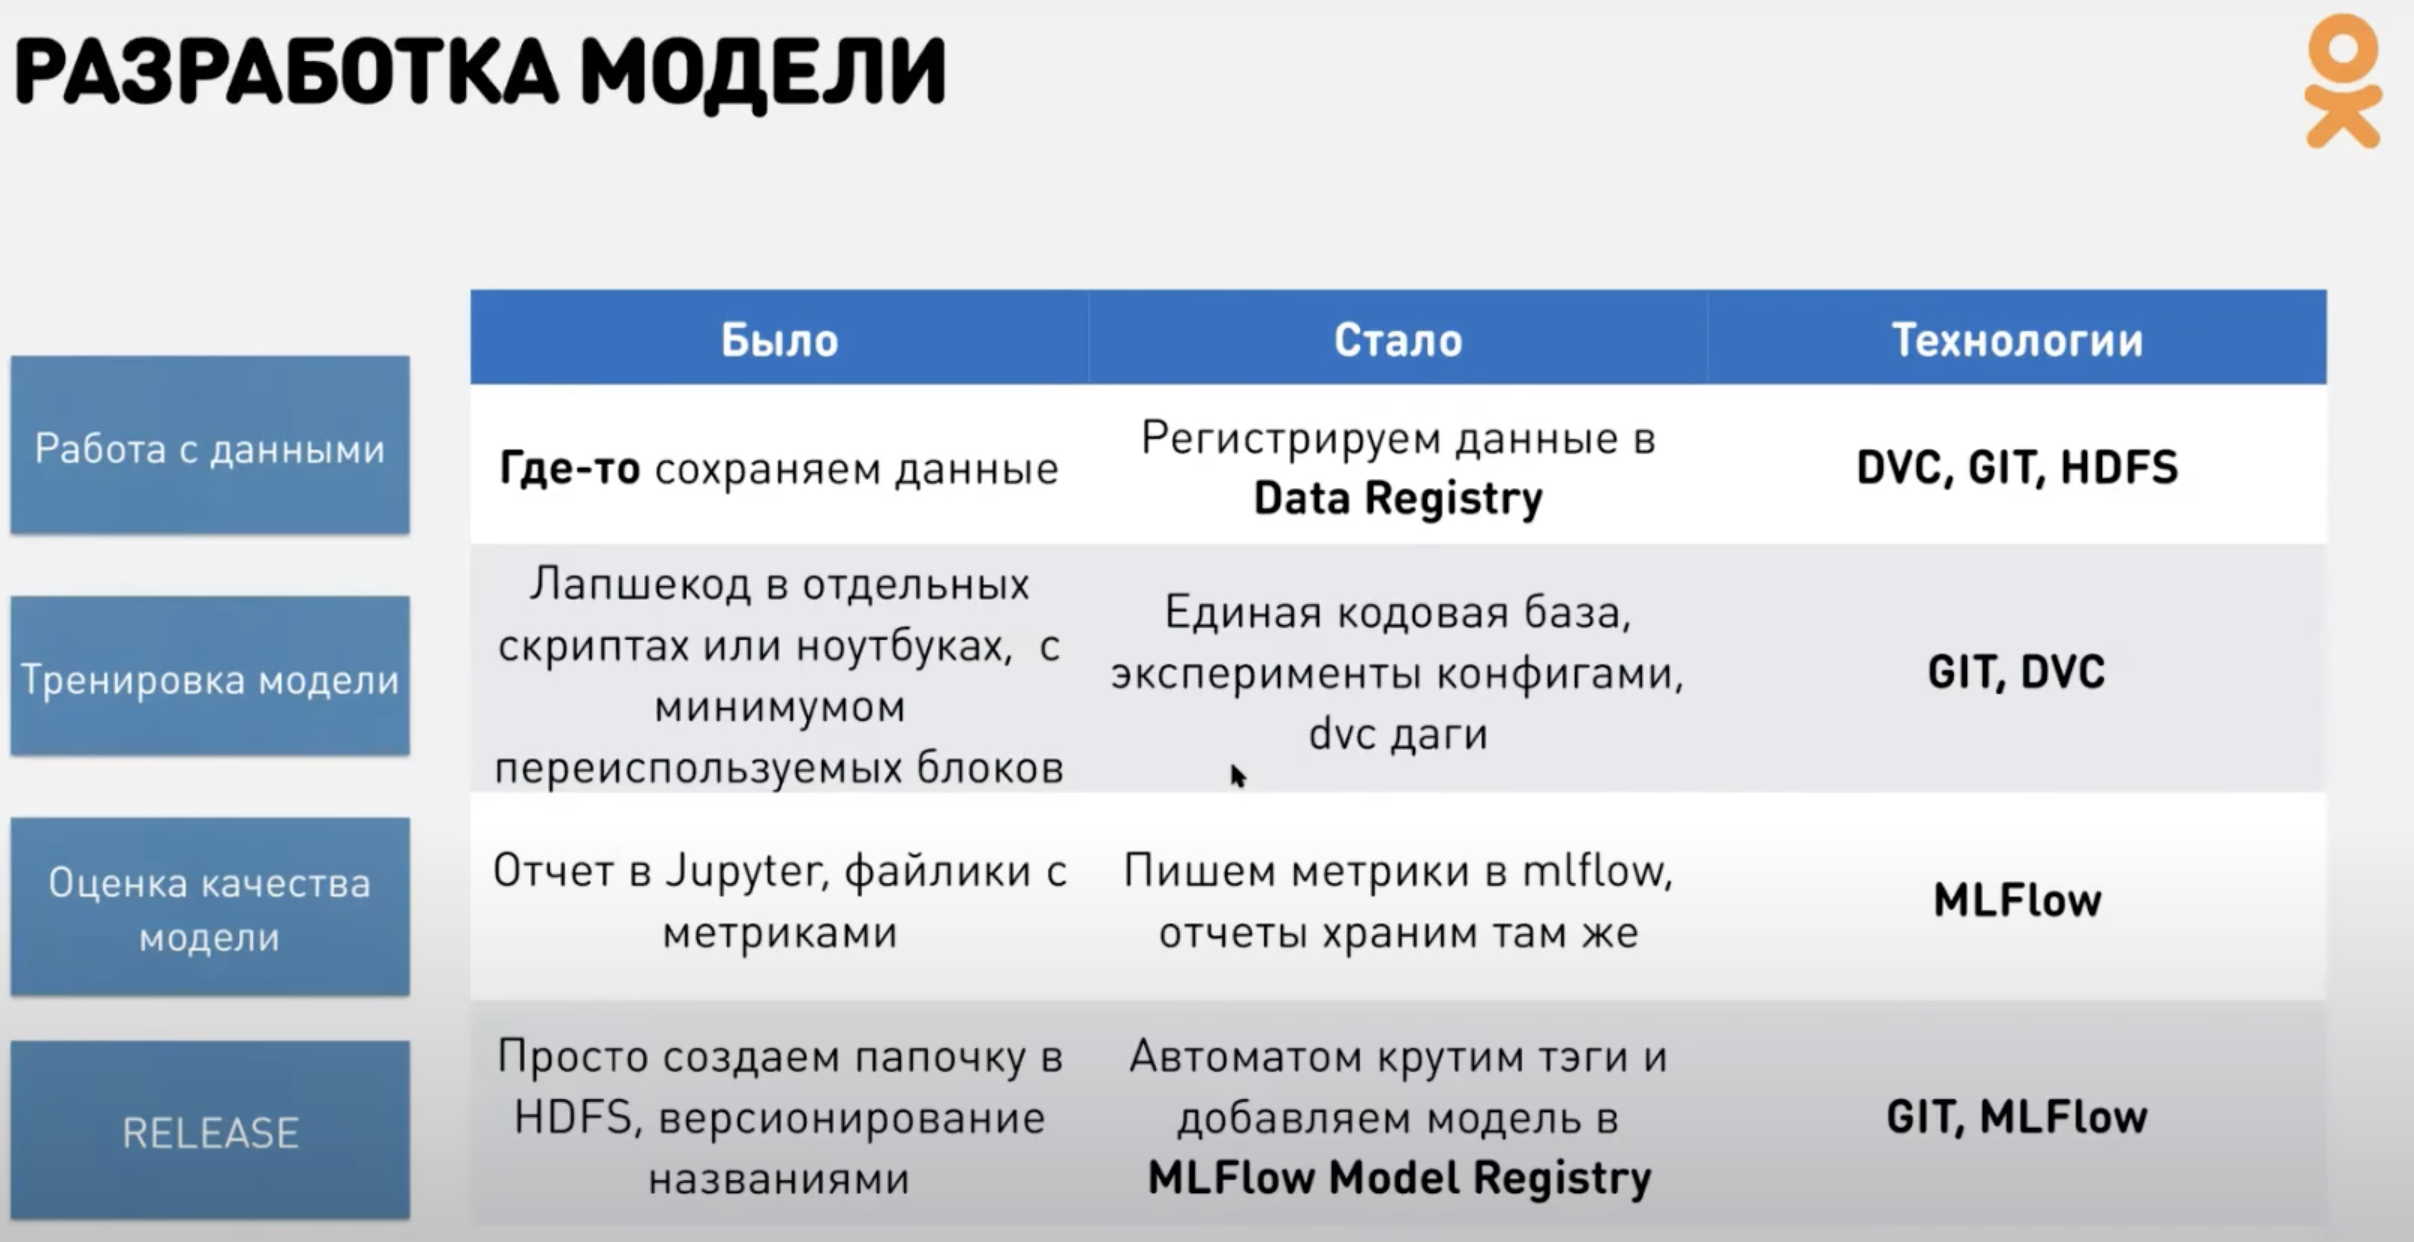
\includegraphics[width=0.9\linewidth]{images/ok_repa.png}
    \label{fig:ok_repa}
\end{figure}

Используют DVC для работы с hdfs файлами в том числе.

\section{Comparison of frameworks for pipelines automation: Airflow vs. Prefect}

\textbf{Video:}~\url{https://youtu.be/Qx09k-bmdBU} \\

Prefect\footnote{\url{https://github.com/PrefectHQ/prefect}} - так же как и Airflow, является инструсментом для автоматизации пайплайнов.
Был создан основными контрибьютерами Airflow. \\

Прямо из доклада не очень понятно, почему Prefect лучше чем Airflow, но на medium'e есть большой пост\footnote{\url{https://medium.com/the-prefect-blog/why-not-airflow-4cfa423299c4}} от авторов Prefect про преимущества в сравнении с Airflow

Самое очевидное улучшение - более понятный и приятный UI.

\section{[MTS] Testing for Data Science Hands-on Guide}
\label{sec:testing_ds}

\textbf{Video:}~\url{https://youtu.be/GgL4BKWYlx8} 

\textbf{Code:}~\url{https://gitlab.com/Julia_chan/testing-for-data-science} \\



\spacerule

\dbox{\textbf{Key Takeaways:}
\begin{enumerate}
    \item Продолжать использовать \href{https://paper.dropbox.com/doc/Reproducible-Research-Draft--A7_r_i5_5DxZO4k9GQMzGWu3AQ-AfvEwFDcTF6lG0nWrdPWj}{рекомендации} (не забывать про code-review)
    \item Подумать над тем, чтобы создать Feature Store (пример: то как организовано хранение признаков в хадупе Mail.ru)
    \item Попробовать посмотреть на DVC + hdfs
\end{enumerate}}

\spacerule

\section*{Управление DS проектами}

Использование Kanban в DataScience команде:

\url{https://drive.google.com/file/d/1fXJlM_sdSQTc8kXI8aMIftTCHZj2_AhG/view}.

(к сожалению только презентация без видео)